\documentclass[10pt,a4paper, margin=1in]{article}
\usepackage{fullpage}
\usepackage{amsfonts, amsmath, pifont}
\usepackage{amsthm}
\usepackage{graphicx}
\usepackage{float}

\usepackage{tkz-euclide}
\usepackage{tikz}
\usepackage{pgfplots}
\usetikzlibrary{angles, quotes}
\pgfplotsset{compat=1.13}

\usepackage{geometry}
 \geometry{
 a4paper,
 total={210mm,297mm},
 left=10mm,
 right=10mm,
 top=10mm,
 bottom=12mm,
 }

 \begin{filecontents}{q3a.dat}
 n   xn
 2  0
 1  1
 0   0
 -1   0
 -2   -2
 -3   0
 -4   3
 -5   0
 -6   0
 -7   -4
 -8   0
 -9   5
 -10  0
 -11  6
 -12  0
\end{filecontents}

\begin{filecontents}{q3b.dat}
 n   xn
-1  0
 0  1
 1   0
 2   0
 3   -2
 4   0
 5   3
 6   0
 7   0
 8   -4
 9   0
 10   5
 11  0
 12  6
 13  0
\end{filecontents}
\begin{filecontents}{q3c.dat}
 n   xn
-1  0
 0  1
 1   0
 2   0
 3   0
 4   -4
 5   5
 6   6
 7   0
\end{filecontents}
\begin{filecontents}{q3d.dat}
 n   xn
 7  0
 6  6
 5  5
 4  -4
 3  0
 2  0
 1  1
 0   1
 -1   0
 -2   -2
 -3   0
 -4   3
 -5   0
 -6   0
 -7   -4
 -8   0
 -9   5
 -10  0
 -11  6
 -12  0
\end{filecontents}

 % Write both of your names here. Fill exxxxxxx with your ceng mail address.
 \author{
  Goksel, Furkan\\
  \texttt{e2237436@ceng.metu.edu.tr}
  \and
  Gursoy, Ceren\\
  \texttt{e2237485@ceng.metu.edu.tr}
}
\title{CENG 384 - Signals and Systems for Computer Engineers \\
Spring 2020 \\
Written Assignment 1}
\begin{document}
\maketitle



\noindent\rule{19cm}{1.2pt}

\begin{enumerate}

\item
    \begin{enumerate}
    % Write your solutions in the following items.
    \item
    We know that rectangular form of any complex number is $z=x+yj$, and conjugate of any complex number is  $\bar{z}=x-yj$. \\
    Therefore, if we replace z and $\bar{z}$ in given equation we get, $x+1+yj = -3x+(3y+1)j$ \\
    When two complex numbers are equal, their real and imaginary parts are same. From this fact we get, $x+1=-3x$ and $3y+1=y$\\
    $x=\frac{-1}{4}$, $y=\frac{-1}{2}$ . So, $z=-\frac{1}{4}-\frac{1}{2}j$\\\\
    i) Magnitude of any complex number is calculated as $|z| = \sqrt{x^2+y^2}$. So, $|z|^2 = x^2+y^2= \frac{1}{16}+\frac{1}{4}=\frac{5}{16}$\\\\
    ii)\\ \begin{tikzpicture}[
            every edge quotes/.append style = {anchor=south, sloped}
                        ]
            % axis
            \draw[thick, ->] (0.35,0) -- (-5.5,0) coordinate[label=above: Re] (x);
            \draw[thick, ->] (0,0.35) -- (0,-5.5)
            node[right] {Im}
            node[below right=5mm] {$Z=-\frac{1}{4}-\frac{1}{2}j$};
            \coordinate[label=below right:$ O $] (O);
            % phasor
            \fill           (-3.5,-3) coordinate[label=below left:$Z$] (z) circle(0.05);
            \draw[dashed]   (0,-3) node[right] {$-\frac{1}{2}$} -| (-3.5,0) node[above] {$-\frac{1}{4}$};
            \draw[thick]    (O) to ["$|Z|=\frac{\sqrt{5}}{4}$"] (-3.5,-3);
            % angle
            \pic [draw, <->,angle radius=11mm, angle eccentricity=1.2,"$\theta$"] {angle = x--O--z};
    \end{tikzpicture} \\
        Where $\theta$ is $tan^{-1}(2)$ \\ \\
    \item For given $z=re^{j\theta}$ , $z^2=25j$ \\
    We know that any complex number in polar form is equal to $z=re^{j\theta}=r(cos\theta+jsin\theta)$ (Using Euler Equation). Therefore, if we calculate $z^2$ we get:
    \begin{gather*}
        z^2 =(r(cos\theta+jsin\theta))^2= r^2(cos^2\theta+jcos\theta sin\theta + jcos\theta sin\theta - sin^2\theta) = 25j
    \end{gather*} \\
    Since Real part of Z is $0$, $cos^2\theta- sin^2\theta = 0$, and using $cos^2\theta + sin^2\theta = 1$ from our trigonometry knowledge, if we add them side by side we get:
    \begin{gather*}
        2cos^2\theta = 1 \rightarrow cos\theta=\frac{+1}{\sqrt{2}}\text{ or } \frac{-1}{\sqrt{2}}
    \end{gather*}\\
    and \begin{gather*}
        \theta = \frac{\pi}{4} \text{ , } \frac{3\pi}{4}
        \text{ , } \frac{5\pi}{4}
        \text{ or } \frac{7\pi}{4}
    \end{gather*}\\
    From imaginary part, we know that:
    \begin{gather*}
        (2r^2cos\theta sin\theta )j= 25j \\
    \end{gather*} \\
    $r^2$ can not be negative, so both of $sin\theta$ and $cos\theta$ must be positive or negative. Therefore, $\theta$ must be $\frac{\pi}{4}$ or $\frac{5\pi}{4}$.
     \begin{gather*}
        2r^2\frac{1}{\sqrt{2}}\frac{1}{\sqrt{2}} = 25 \\
        r^2=25 \rightarrow r=5
    \end{gather*} \\
    So, z in polar form: $5e^{j\frac{\pi}{4}}$ or $5e^{j\frac{5\pi}{4}}$
    \item For given $z=\dfrac{(1+j)(1-\sqrt{3}j)}{1-j}$\\
    We can find magnitude and angle of z using following formulas:
    \begin{gather*}
        |z_1z_2|=|z_1||z_2| \\
        |\dfrac{z_1}{z_2}| = \dfrac{|z_1|}{|z_2|} \\
        \angle \{z_1z_2\}=\angle \{z_1\} + \angle \{z_2\} \\
        \angle \{\dfrac{z_1}{z_2}\}=\angle \{z_1\} + \angle \{z_2\}
    \end{gather*} \\
    Independently, magnitude of $1+j$ is $\sqrt{2}$, magnitude of $1-\sqrt{3}j$ is 2, and magnitude of $1-j$ is $\sqrt{2}$. \\ \\Using above formulas, magnitude of z calculated like following:
    \begin{gather*}
        |z|=\dfrac{\sqrt{2}*2}{\sqrt{2}}=2
    \end{gather*}
    Independently, their  angles are $\angle (1+j) = tan^{-1}1 = \frac{\pi}{4}$, $\angle (1-\sqrt{3}j) = tan^{-1}({\frac{-\sqrt{3}}{1}}) = \frac{-\pi}{3}$ and $\angle (1-j) = tan^{-1}(-1) = \frac{-\pi}{4}$. \\\\
    Using above formulas, angle of z calculated like following:
    \begin{gather*}
        \angle z = \frac{\pi}{4} - \frac{\pi}{3} + \frac{\pi}{4} = \frac{\pi}{6}
    \end{gather*}

    \item For given $z=je^{-j\frac{\pi}{2}}$,\\
    It is not in the polar form, actually it is the multiplication of two complex number which are $z_1=j$ and $z_2=e^{-\frac{\pi}{2}j}$. \\
    If we write $z_1$ in polar form:
    \begin{gather*}
        j=0+j=cos\frac{\pi}{2}+jsin\frac{\pi}{2}=e^{\frac{\pi}{2}j}
    \end{gather*} \\
    Therefore for polar form of z:
    \begin{gather*}
       e^{\frac{\pi}{2}j}*e^{-\frac{\pi}{2}j} = e^0 = 1
    \end{gather*}

    \end{enumerate}


\item %write the solution of q2
First of all, in order to draw $\dfrac{1}{2}x(2t-2)$, we should move on step by step, and we should find $x(t-2)$, $x(2t-2)$, $\dfrac{1}{2}x(2t-2)$ in that order. \\ \\
In order to draw $x(t-2)$ we need to shift this graph 2 unit to the right:\clearpage
\begin{figure}[ht!]
    \centering
        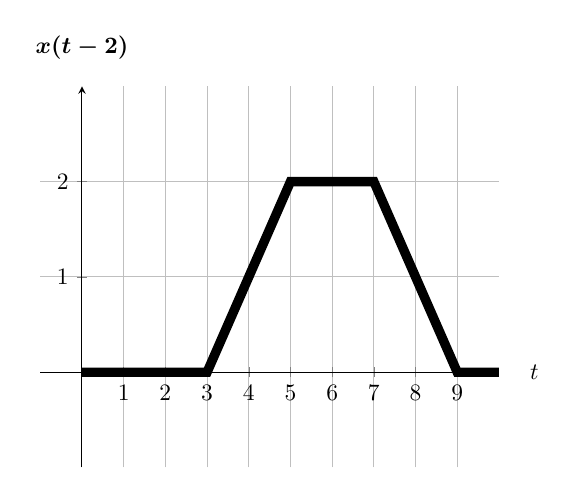
\begin{tikzpicture}[scale=0.85]
           \begin{axis}[
          axis lines=middle,
          xlabel={$t$},
          ylabel={$\boldsymbol{x(t-2)}$},
          xtick={0, 1, 2, 3, ..., 9},
          ytick={0, 1, 2},
          ymin=-1, ymax=3,
          xmin=-1, xmax=10,
          every axis x label/.style={at={(ticklabel* cs:1.05)}, anchor=west,},
          every axis y label/.style={at={(ticklabel* cs:1.05)}, anchor=south,},
          grid,
        ]
           \path[draw,line width=4pt] (0,0) -- (3,0) -- (5,2) -- (7,2) -- (9,0) -- (10,0);
           \end{axis}
        \end{tikzpicture}
        \caption{$t$ vs. $x(t-2)$.}
        \label{fig:q2}
\end{figure}

Then we scale it by 2 (divide values on the x axis by 2, eg. graph will start at $\dfrac{3}{2}=1.5$ now) and we get $x(2t-2)$: \\

\begin{figure}[ht!]
    \centering
        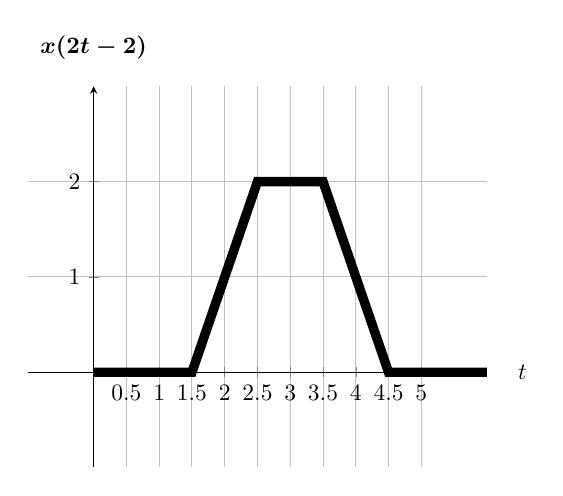
\begin{tikzpicture}[scale=0.85]
           \begin{axis}[
          axis lines=middle,
          xlabel={$t$},
          ylabel={$\boldsymbol{x(2t-2)}$},
          xtick={0, 0.5, 1, 1.5, 2, 2.5, 3, 3.5, ..., 5},
          ytick={0, 1, 2},
          ymin=-1, ymax=3,
          xmin=-1, xmax=6,
          every axis x label/.style={at={(ticklabel* cs:1.05)}, anchor=west,},
          every axis y label/.style={at={(ticklabel* cs:1.05)}, anchor=south,},
          grid,
        ]
           \path[draw,line width=4pt] (0,0) -- (1.5,0) -- (2.5,2) -- (3.5,2) -- (4.5,0) -- (6,0);
           \end{axis}
        \end{tikzpicture}
        \caption{$t$ vs. $x(2t-2)$.}
        \label{fig:q3}
\end{figure}
\leavevmode \\

Now, to obtain $\dfrac{1}{2}x(2t-2)$, we just divide values on the y axis by 2:
\begin{figure}[ht!]
    \centering
        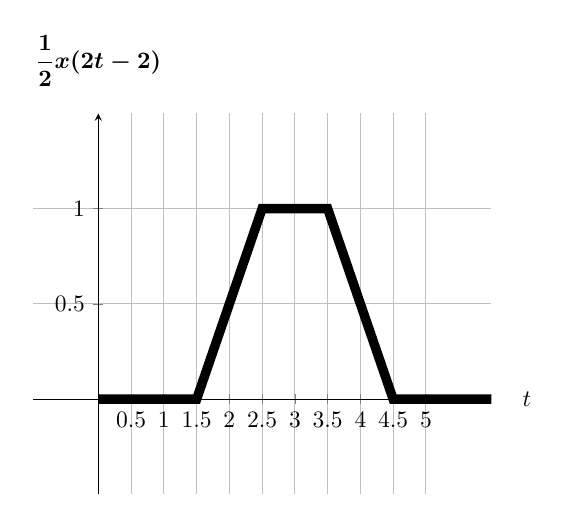
\begin{tikzpicture}[scale=0.85]
           \begin{axis}[
          axis lines=middle,
          xlabel={$t$},
          ylabel={$\boldsymbol{\dfrac{1}{2}x(2t-2)}$},
          xtick={0, 0.5, 1, 1.5, 2, 2.5, 3, 3.5, ..., 5},
          ytick={0, 0.5, 1},
          ymin=-0.5, ymax=1.5,
          xmin=-1, xmax=6,
          every axis x label/.style={at={(ticklabel* cs:1.05)}, anchor=west,},
          every axis y label/.style={at={(ticklabel* cs:1.05)}, anchor=south,},
          grid,
        ]
           \path[draw,line width=4pt] (0,0) -- (1.5,0) -- (2.5,1) -- (3.5,1) -- (4.5,0) -- (6,0);
           \end{axis}
        \end{tikzpicture}
        \caption{$t$ vs. $\dfrac{1}{2}x(2t-2)$.}
        \label{fig:q4}
\end{figure}
\item
    \begin{enumerate}
    \item
    Again, we should move on step by step: \\ \\
    In order to find and draw x[-n], we use reflection (take the symmetry of x[n] with respect to y axis): \clearpage
    \begin{figure} [ht!]
    \centering
    \begin{tikzpicture}[scale=0.95]
      \begin{axis}[
          axis lines=middle,
          xlabel={$n$},
          ylabel={$\boldsymbol{x[-n]}$},
          xtick={ -12, -11, -10,  ..., 2},
          ytick={-4, -3, -2, -1, ..., 6},
          ymin=-4, ymax=6,
          xmin=-12, xmax=2,
          every axis x label/.style={at={(ticklabel* cs:1.05)}, anchor=west,},
          every axis y label/.style={at={(ticklabel* cs:1.05)}, anchor=south,},
          grid,
        ]
        \addplot [ycomb, black, thick, mark=*] table [x={n}, y={xn}] {q3a.dat};
      \end{axis}
    \end{tikzpicture}
    \caption{$n$ vs. $x[-n]$.}
    \label{fig:q5}
\end{figure}
In order to find x[2n-1], firstly, shift x[n] 1 unit to the right and we get x[n-1]:
    \begin{figure} [ht!]
    \centering
    \begin{tikzpicture}[scale=0.95]
      \begin{axis}[
          axis lines=middle,
          xlabel={$n$},
          ylabel={$\boldsymbol{x[n-1]}$},
          xtick={ -1, 0,  ..., 13},
          ytick={-4, -3, -2, -1, ..., 6},
          ymin=-4, ymax=6,
          xmin=-1, xmax=13,
          every axis x label/.style={at={(ticklabel* cs:1.05)}, anchor=west,},
          every axis y label/.style={at={(ticklabel* cs:1.05)}, anchor=south,},
          grid,
        ]
        \addplot [ycomb, black, thick, mark=*] table [x={n}, y={xn}] {q3b.dat};
      \end{axis}
    \end{tikzpicture}
    \caption{$n$ vs. $x[n-1]$.}
    \label{fig:q6}
\end{figure} \\
Now we can scale it by 2, and we can get x[2n-1] (some values can lost because it is discrete time signal and in discrete time signal time values that are not integers are undefined): \\
    \begin{figure} [ht!]
    \centering
    \begin{tikzpicture}[scale=0.95]
      \begin{axis}[
          axis lines=middle,
          xlabel={$n$},
          ylabel={$\boldsymbol{x[2n-1]}$},
          xtick={ -1, 0,  ..., 6},
          ytick={-4, -3, -2, -1, ..., 6},
          ymin=-4, ymax=6,
          xmin=-1, xmax=6,
          every axis x label/.style={at={(ticklabel* cs:1.05)}, anchor=west,},
          every axis y label/.style={at={(ticklabel* cs:1.05)}, anchor=south,},
          grid,
        ]
        \addplot [ycomb, black, thick, mark=*] table [x={n}, y={xn}] {q3c.dat};
      \end{axis}
    \end{tikzpicture}
    \caption{$n$ vs. $x[2n-1]$.}
    \label{fig:q7}
\end{figure} \clearpage
Now we got x[2n-1] and x[-n], all that's left is to adding these two signals:
    \begin{figure} [ht!]
    \centering
    \begin{tikzpicture}[scale=1.2]
      \begin{axis}[
          axis lines=middle,
          xlabel={$n$},
          ylabel={$\boldsymbol{x[-n]+x[2n-1]}$},
          xtick={ -12,-11,-10,  ..., 6},
          ytick={-4, -3, -2, -1, ..., 6},
          ymin=-4, ymax=6,
          xmin=-12, xmax=6,
          every axis x label/.style={at={(ticklabel* cs:1.05)}, anchor=west,},
          every axis y label/.style={at={(ticklabel* cs:1.05)}, anchor=south,},
          grid,
        ]
        \addplot [ycomb, black, thick, mark=*] table [x={n}, y={xn}] {q3d.dat};
      \end{axis}
    \end{tikzpicture}
    \caption{$n$ vs. $x[-n]+x[2n-1]$.}
    \label{fig:q8}
\end{figure} \\
    \item Unit impulse function $\delta$ is a function such that it's value is 1 at n=0 and otherwise it is 0. Therefore we can express $x[-n]+x[2n-1]$ by using shifted impulse functions.It is expressed as following: \\ \\
    $6 \delta [n+11]+ 5 \delta [n+9] -4 \delta [n+7] +3 \delta [n+4] -2 \delta [n+2] + \delta [n] +\delta [n-1] -4 \delta [n-4] + 5 \delta [n-5] +6 \delta [n-6]$
    \end{enumerate}

\item
    \begin{enumerate}
    \item
    %write the solution of q4a
    Firstly, we calculate their periods independently:
    To find the period of $7sin[\frac{5\pi}{8}n-\frac{2\pi}{3}]$, \\
    \begin{gather*}
        x[n] = x[n+N] \\
        7sin[\frac{5\pi}{8}(n+N)-\frac{2\pi}{3}]=7sin[\frac{5\pi}{8}n+\frac{5\pi}{8}N-\frac{2\pi}{3}]
    \end{gather*} \\
    If this discrete time signal is periodic, we can find integers $N>0,k$ for following $\frac{5\pi}{8}N=2\pi k$ and N is fundamental period for smallest possible k, then for $k=5$, we get $N=16$ and fundamental period is 16. \\ \\ Similarly for $2cos[\frac{2\pi}{3}n]$,
    \begin{gather*}
        x[n] = x[n+N] \\
        2cos[\frac{2\pi}{3}(n+N)]=2cos[\frac{2\pi}{3}n+\frac{2\pi}{3}N]
    \end{gather*} \\
    If this discrete time signal is periodic, we can find integers $N>0,k$ for following $\frac{2\pi}{3}N=2\pi k$ and N is fundamental period for smallest possible k, then for $k=1$, we get $N=3$ and fundamental period is 3. \\ \\
    Hence, it is periodic and overall fundamental period must be their least common multiplier which is 48.
    \item %write the solution of q4b
    If given signal is periodic:
    \begin{gather*}
        x[n] = x[n+N] \\
        3cos[5(n+N)-\frac{3\pi}{4}] = 3cos[5n+5N-\frac{3\pi}{4}]
    \end{gather*} \\
    We should find integers $N>0,k$ for following $5N=2\pi k$. However, it is not possible to find an integer N. So, this signal is not periodic.
    \item %write the solution of q4c
    If given signal is periodic:
    \begin{gather*}
         x(t) = x(t+T) \\
         4sin(5\pi(t+T)-\frac{3\pi}{5}) = 4sin(5\pi t+5\pi T-\frac{3\pi}{5})
    \end{gather*} \\
    For fundamental period, $5\pi T=2\pi$ , so fundamental period $T=\frac{2}{5}$, and it is periodic.
    \item %write the solution of q4d
    If given signal is periodic:
    \begin{gather*}
        je^{j2t} = je^{j2(t+T)} = je^{j2t+j2T}=je^{j2t}e^{j2T} \text{(If we divide both side to $e^{j2t})$}\\
        1 =e^{j2T}
    \end{gather*} \\
    From Euler equation, $e^{j2T}=cos2T+jsin2T$, then $1=cos2T+jsin2T$. If we solve it, $cos2T=1$, and $jsin2T=0$, T will be $\pi$. Therefore it is periodic, and fundamental period is $\pi$
    \end{enumerate}

\item %write the solution of q5
By definition for continuous time signals,\\
\begin{gather*}
    \text{A signal is odd if x(t) = -x(-t) for  }\forall t   \\
    \text{A signal is even if x(t) = x(-t) for   } \forall t
\end{gather*} \\
Therefore finding just one counterexample is enough to show this signal is not odd or even. For example, we know that x(3) = 2 and x(-3) = 0 (assuming not drawn parts are equal to 0), it proves this signal is neither odd nor even since $x(3) \neq x(-3)$ and $x(3) \neq -x(-3)$. \\
Any signal can be decomposed into even and odd part,\\
\begin{gather*}
    \text{Ev\{x(t)\}}=\dfrac{x(t)+x(-t)}{2} \\
    \text{Odd\{x(t)\}}=\dfrac{x(t)-x(-t)}{2}
\end{gather*}
We can also express x(t) like following: \\
\[ \begin{cases}
      0 & t\leq 1 \\
      t-1 & 1\leq t\leq 3 \\
      2 & 3\leq t \leq 5 \\
      7-t & 5\leq t \leq7 \\
      0 &  7 \leq t

   \end{cases}
\]
Then we can also express x(-t) like following: (It is just reflection): \\
\[ \begin{cases}
    0 &  t \leq -7 \\
    7+t & -7 \leq t \leq -5 \\
     2 & -5\leq t \leq -3 \\
     -t-1 & -3\leq t\leq -1 \\
      0 & -1\leq t
   \end{cases}
\]
We can also draw x(-t):
\begin{figure}[ht!]
    \centering
        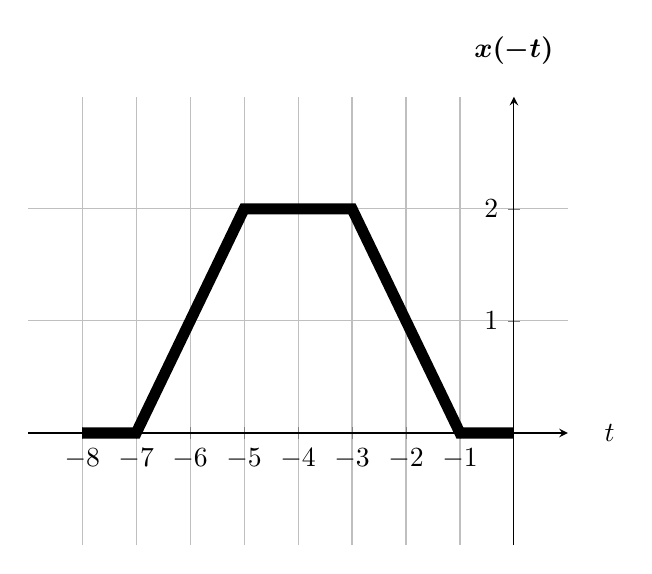
\begin{tikzpicture}[scale=1.0]
           \begin{axis}[
          axis lines=middle,
          xlabel={$t$},
          ylabel={$\boldsymbol{x(-t)}$},
          xtick={0, -1, -2, -3, ..., -8},
          ytick={0, 1, 2},
          ymin=-1, ymax=3,
          xmin=-9, xmax=1,
          every axis x label/.style={at={(ticklabel* cs:1.05)}, anchor=west,},
          every axis y label/.style={at={(ticklabel* cs:1.05)}, anchor=south,},
          grid,
        ]
           \path[draw,line width=4pt] (0,0) -- (-1,0) -- (-3,2) -- (-5,2) -- (-7,0) -- (-8,0);
           \end{axis}
        \end{tikzpicture}
        \caption{$t$ vs. $x(-t)$.}
        \label{fig:q9}
    \end{figure} \\
    Now for even part we add these two signals and divide by two. Ev\{x(t)\}:
    \[ \begin{cases}
    0 &  t \leq -7 \\
    \dfrac{7+t}{2} & -7 \leq t \leq -5 \\
     1 & -5\leq t \leq -3 \\
     \dfrac{-t-1}{2} & -3\leq t\leq -1 \\
      0 & -1\leq t \leq 1 \\
      \dfrac{t-1}{2} & 1\leq t\leq 3 \\
      1 & 3\leq t \leq 5 \\
      \dfrac{7-t}{2} & 5\leq t \leq7 \\
      0 &  7 \leq t
   \end{cases}
\]
And draw the even part Ev\{x(t)\}:
\begin{figure}[ht!]
    \centering
        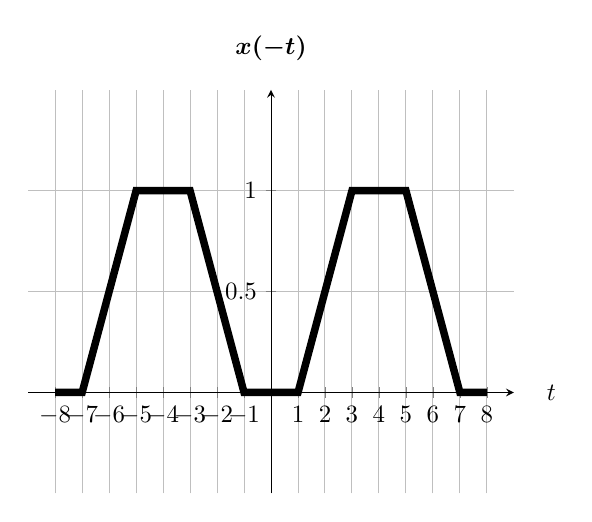
\begin{tikzpicture}[scale=0.90]
           \begin{axis}[
          axis lines=middle,
          xlabel={$t$},
          ylabel={$\boldsymbol{x(-t)}$},
          xtick={-8, -7, -6, ..., 8},
          ytick={0, 0.5, 1},
          ymin=-0.5, ymax=1.5,
          xmin=-9, xmax=9,
          every axis x label/.style={at={(ticklabel* cs:1.05)}, anchor=west,},
          every axis y label/.style={at={(ticklabel* cs:1.05)}, anchor=south,},
          grid,
        ]
           \path[draw,line width=3pt] (-8,0) -- (-7,0) -- (-5,1) -- (-3,1) --(-1,0) -- (1,0) -- (3,1) -- (5,1) -- (7,0) -- (8,0);
           \end{axis}
        \end{tikzpicture}
        \caption{$t$ vs. $x(-t)$.}
        \label{fig:q10}
    \end{figure} \\ \\
    Now for odd part we subtract x(-t) from x(t) and divide by two. Odd\{x(t)\}:
    \[ \begin{cases}
    0 &  t \leq -7 \\
    \dfrac{-7-t}{2} & -7 \leq t \leq -5 \\
     -1 & -5\leq t \leq -3 \\
     \dfrac{t+1}{2} & -3\leq t\leq -1 \\
      0 & -1\leq t \leq 1 \\
      \dfrac{t-1}{2} & 1\leq t\leq 3 \\
      1 & 3\leq t \leq 5 \\
      \dfrac{7-t}{2} & 5\leq t \leq7 \\
      0 &  7 \leq t
   \end{cases}
\]
\clearpage
And finally draw the the odd part, odd\{x(t)\}:
\begin{figure}[ht!]
    \centering
        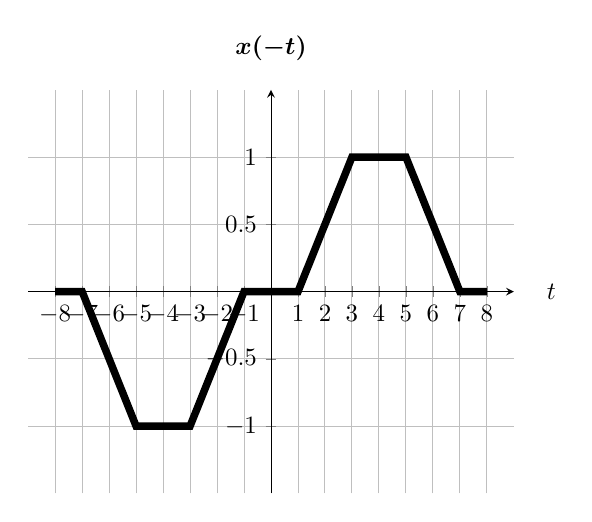
\begin{tikzpicture}[scale=0.90]
           \begin{axis}[
          axis lines=middle,
          xlabel={$t$},
          ylabel={$\boldsymbol{x(-t)}$},
          xtick={-8, -7, -6, ..., 8},
          ytick={-1,-0.5, 0, 0.5, 1},
          ymin=-1.5, ymax=1.5,
          xmin=-9, xmax=9,
          every axis x label/.style={at={(ticklabel* cs:1.05)}, anchor=west,},
          every axis y label/.style={at={(ticklabel* cs:1.05)}, anchor=south,},
          grid,
        ]
           \path[draw,line width=3pt] (-8,0) -- (-7,0) -- (-5,-1) -- (-3,-1) --(-1,0) -- (1,0) -- (3,1) -- (5,1) -- (7,0) -- (8,0);
           \end{axis}
        \end{tikzpicture}
        \caption{$t$ vs. $x(-t)$.}
        \label{fig:q11}
    \end{figure} \\
\item
    \begin{enumerate}
    \item %write the solution of q6a
    Unit step function u(t) is 1 for $t> 0$, and 0 for $t < 0$, Using this fact given signal can be written using unit step functions:
    \begin{gather*}
        x(t) = u(t-1)-3u(t-3)+4u(t-4)
    \end{gather*}
    \item %write the solution of q6b
    We know that (from Oppenheim book):
    \begin{gather*}
        Ku(t) = \int_{-\infty}^{t} K\delta(T) dT \\
        K\delta(t)=K\dfrac{du(t)}{dt}
    \end{gather*}
    Then using these formulas, we can find:
    \begin{gather*}
        \dfrac{dx(t)}{dt} = \delta(t-1)-3\delta(t-3)+4\delta(t-4)
    \end{gather*}
    And if we draw it:
    \begin{figure} [ht!]
    \centering
    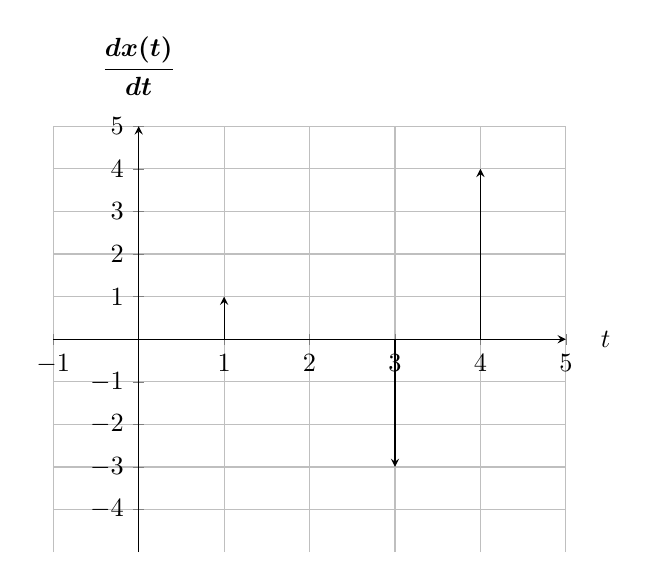
\begin{tikzpicture}[scale=0.95]
      \begin{axis}[
          axis lines=middle,
          xlabel={$t$},
          ylabel={$\boldsymbol{\dfrac{dx(t)}{dt}}$},
          xtick={ -1, 0,  ..., 5},
          ytick={-4, -3, -2, -1, ..., 5},
          ymin=-5, ymax=5,
          xmin=-1, xmax=5,
          every axis x label/.style={at={(ticklabel* cs:1.05)}, anchor=west,},
          every axis y label/.style={at={(ticklabel* cs:1.05)}, anchor=south,},
          grid,
        ]
        \draw [black, -stealth] (1,0.0) -- (1,1.0);
        \draw [black, -stealth] (3,0.0) -- (3,-3.0);
        \draw [black, -stealth] (4,0.0) -- (4,4.0);
      \end{axis}
    \end{tikzpicture}
    \caption{$t$ vs. $\dfrac{dx(t)}{dt}$.}
    \label{fig:q12}
\end{figure} \\
    \end{enumerate}

\end{enumerate}
\end{document}
